\documentclass[tikz,border=10pt]{standalone}
\usepackage[utf8]{inputenc}
\usepackage{tikz}
\usepackage{tikz-3dplot}
\usepackage{amsmath}

\usetikzlibrary{arrows.meta, calc, positioning, shapes.geometric, decorations.markings, backgrounds}

\begin{document}

\tdplotsetmaincoords{70}{110} % Set viewing angle (theta, phi)

\begin{tikzpicture}[
    scale=1.5,
    tdplot_main_coords,
    font=\sffamily,
    >=Stealth,
    % Trajectory styles
    swing/.style={color=purple, line width=1.2pt, postaction={decorate, decoration={markings, mark=at position 0.3 with {\arrow{>}}, mark=at position 0.7 with {\arrow{>}}}}},
    stance/.style={color=purple, line width=1.2pt, postaction={decorate, decoration={markings, mark=at position 0.5 with {\arrow{<}}}}},
    % Dimension styles
    dim/.style={color=orange, line width=0.8pt},
    dimlabel/.style={rectangle, draw=orange, fill=white, rounded corners=2pt, inner sep=2pt, font=\sffamily\small, text=red!80!black},
    % Axis styles
    axis/.style={->, thick, black}
]

    % Define parameters
    \def\Lx{4}     % Step length X
    \def\Ly{1.5}   % Step length Y (lateral offset, if any. Let's keep it 0 for the main trajectory to match the image)
    \def\h{2.5}    % Step height
    \def\H{4.0}    % Robot height
    
    % Draw ground plane (dashed)
    \draw[gray, dashed, thin] (-\Lx, -2, 0) -- (\Lx, -2, 0) -- (\Lx, 2, 0) -- (-\Lx, 2, 0) -- cycle;
    \draw[gray, dashed, thin] (-\Lx, 0, 0) -- (\Lx, 0, 0);
    \draw[gray, dashed, thin] (0, -2, 0) -- (0, 2, 0);

    % Draw Axes
    \draw[axis] (0,0,0) -- (3,0,0) node[anchor=north east]{$x$};
    \draw[axis] (0,0,0) -- (0,3,0) node[anchor=north west]{$y$};
    \draw[axis] (0,0,0) -- (0,0,4) node[anchor=south]{$z$};

    % Draw Stance Trajectory (Straight line on ground)
    % Reversing the direction as stance moves body forward, so foot moves backward relative to body
    \draw[stance] (\Lx/2, 0, 0) -- (-\Lx/2, 0, 0);
    
    % Draw Swing Trajectory (Parabola)
    % Parametric equation for parabola: x(t) = t, y(t) = 0, z(t) = h * (1 - (t/(Lx/2))^2)
    \draw[swing] plot[domain=-\Lx/2:\Lx/2, samples=50] (\x, 0, {\h * (1 - (\x/(\Lx/2))^2)});

    % Add dots at endpoints
    \filldraw[purple] (\Lx/2, 0, 0) circle (1.5pt);
    \filldraw[purple] (-\Lx/2, 0, 0) circle (1.5pt);

    % Labels for trajectories
    \node[rectangle, draw=purple, fill=white, rounded corners=2pt, font=\sffamily\small] at (-\Lx/2 - 1, 0, 0.5) {Swing trajectory};
    \node[rectangle, draw=purple, fill=white, rounded corners=2pt, font=\sffamily\small] at (0, 1.5, 0) {Stance trajectory};
    
    % Link labels to paths
    \draw[purple, thin] (-\Lx/2 - 1, 0, 0.5) -- (-\Lx/2, 0, 0);
    \draw[purple, thin] (0, 1.5, 0) -- (0, 0, 0);

    % Dimensions H and h
    \draw[dim, <->] (0, 0, 0) -- (0, 0, \h) node[pos=0.8, right] {\tikz{\node[dimlabel] {h};}};
    
    % For H, move it to the back left to avoid overlapping the leg
    \draw[gray, dashed] (0, 0, \H) -- (-\Lx/2 - 1.5, 0, \H);
    \draw[gray, dashed] (0, 0, 0) -- (-\Lx/2 - 1.5, 0, 0);
    \draw[dim, <->] (-\Lx/2 - 1.2, 0, 0) -- (-\Lx/2 - 1.2, 0, \H) node[midway, left] {\tikz{\node[dimlabel] {H};}};

    % Dimension Lx/2
    \draw[dim, <->] (0, -0.8, 0) -- (\Lx/2, -0.8, 0) node[midway, below] {\tikz{\node[dimlabel] {Lx/2};}};
    \draw[gray, dashed] (\Lx/2, 0, 0) -- (\Lx/2, -1.0, 0);
    \draw[gray, dashed] (0, 0, 0) -- (0, -1.0, 0);
    
    % Insert the leg image
    % anchor=south east places the foot (bottom-right of image) at the origin
    % Adjust coordinates slightly to match the spherical foot exactly at (0,0,0)
    \node[inner sep=0pt, transform shape=false, anchor=south east] at (0.3, 0, 0.15) {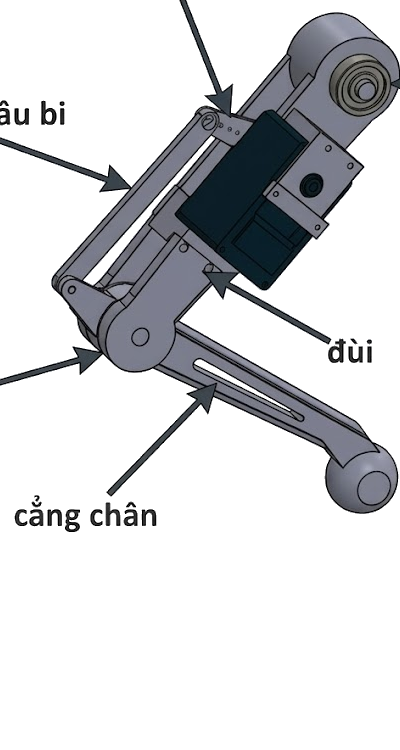
\includegraphics[height=6.5cm]{cropped_leg.png}};

    % Commands Box (placed in 2D space over the 3D plot)
    \begin{scope}[tdplot_screen_coords]
        \node[rectangle, draw=green!50!black, fill=green!10, rounded corners=4pt, inner sep=10pt, align=left, font=\sffamily] 
        at (-4, 2) {
            \textbf{Commands}\\[2mm]
            - Robot\_height : \textcolor{red}{H}\\
            - Step\_height : \textcolor{orange}{h}\\
            - Step\_length\_x : \textcolor{green!50!black}{Lx}\\
            - Step\_length\_y : \textcolor{blue}{Ly}\\
            - Gait\_cycle\_time : \textcolor{purple}{T}\\
            - Gait\_swing\_time : \textcolor{magenta}{tsw}\\
        };
        
        % Arrow from Commands box to the plot
        \draw[ultra thick, fill=green!10, draw=green!50!black] (-2.5, 2.5) -- (-1.8, 2) -- (-2.5, 1.5) -- cycle;
    \end{scope}

\end{tikzpicture}
\end{document}
